\documentclass{ximera}
\title{Images and Graphs}


\begin{document}
\begin{abstract}
    A description of how images and graphs are rendered or included.
\end{abstract}
\maketitle
   
\section*{How Ximera renders Image and Graph Content}

There are several ways to embed graphics into Ximera document. One method is to use \verb|\includegraphics|. Here we see an included a JPEG and a PNG:

\begin{verbatim}
\begin{image}
  %https://commons.wikimedia.org/wiki/File:Lama_LLama_Alpaca_06.jpg
  \includegraphics[width=.3\textwidth]{llama.jpg}\qquad
  %https://commons.wikimedia.org/wiki/File:Llama_in_watercolour.png
  \includegraphics[width=.3\textwidth]{llama.png}
\end{image}
\end{verbatim}
In the code above, the command image is just a Ximera provided wrapper
that can be redefined for printing. It does automatically resize
content though and can be useful for showing images side-by-side:
\begin{image}
  %https://commons.wikimedia.org/wiki/File:Lama_LLama_Alpaca_06.jpg
  \includegraphics[width=.3\textwidth]{llama.jpg}\qquad
  %https://commons.wikimedia.org/wiki/File:Llama_in_watercolour.png
  \includegraphics[width=.3\textwidth]{llama.png}
\end{image}

Here we have a pdf
\begin{center}
  \includegraphics[width=.3\textwidth]{llama.pdf}
\end{center}

Another way to include graphics is to use Tikz. In some sense this is
preferred, as then the source produces the images.
\begin{image}
  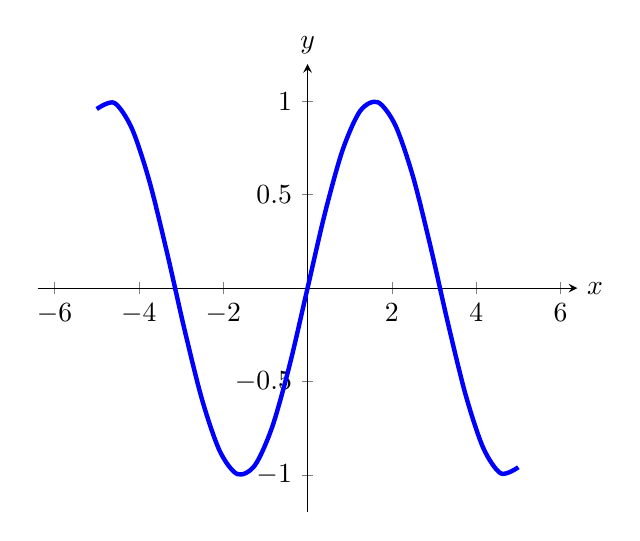
\begin{tikzpicture}
    \begin{axis}[
        xmin=-6.4,
        xmax=6.4,
        ymin=-1.2,
        ymax=1.2,
        axis lines=center,
        xlabel=$x$,
        ylabel=$y$,
        every axis y label/.style={at=(current axis.above origin),anchor=south},
        every axis x label/.style={at=(current axis.right of origin),anchor=west},
      ]
      \addplot [ultra thick, blue, smooth] {sin(deg(x))};
    \end{axis}
  \end{tikzpicture}
\end{image}

\begin{verbatim}
\begin{image}
  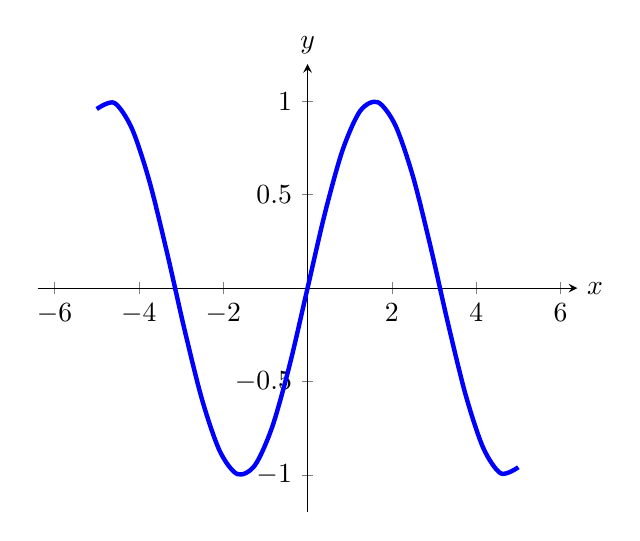
\begin{tikzpicture}
    \begin{axis}[
        xmin=-6.4,
        xmax=6.4,
        ymin=-1.2,
        ymax=1.2,
        axis lines=center,
        xlabel=$x$,
        ylabel=$y$,
        every axis y label/.style={at=(current axis.above origin),anchor=south},
        every axis x label/.style={at=(current axis.right of origin),anchor=west},
      ]
      \addplot [ultra thick, blue, smooth] {sin(deg(x))};
    \end{axis}
  \end{tikzpicture}
\end{image}
\end{verbatim}


    \subsection*{Any Necessary Content}
    
    
    
    \subsection*{Quirks of Rendering}
    
    
    
    \subsection*{Any Ximera-Specific Optional Arguments}
    
    
    
    \subsection*{Accessibility}
    
    
    
    \subsection*{Potential Problems and Pitfalls}
    
    
    
    \subsection*{Any Best Practices or Advice}
    
    

    
\end{document}
